\documentclass[]{article}
\usepackage[utf8]{inputenc}
\usepackage{graphicx}
\usepackage{cancel}
\usepackage{emptypage}
\usepackage{subcaption}
\usepackage{hyperref}
\usepackage{url}
\usepackage{mathrsfs}
\usepackage{amsmath}
\usepackage{amsfonts}
\usepackage{ amssymb }
\usepackage{mathcomp}
\usepackage{gensymb}
\usepackage{tensor}
\usepackage{tcolorbox}
\usepackage{lmodern}
\usepackage{wasysym}
\usepackage{enumerate}
\setlength{\parindent}{2.0em}
\setlength{\parskip}{0.6em}
\renewcommand{\baselinestretch}{1.25}

\usepackage{geometry}
\geometry{
	a4paper,
	total={170mm,257mm},
	left=35mm,
	right=35mm,
	top=25mm,
}
%opening
\title{Recovery of redshift data - DESI}
\author{Sergio Daivd Lobo Bolaño}

\begin{document}

\maketitle

\begin{abstract}
DESI (Dark Energy Spectroscopic Instrument) uses a simulated survey of mock galaxies to compare their redshifts with the -also simulated- redshift measurements of DESI. In this monograph we apply machine learning (ML) methods to the simulation data of DESI to recover the true redshift measurements of the Bright Galaxy Sample using observational variables as input, obtaining a $r^2 = 0.98$ using kernel and ensemble methods. 
\end{abstract}

\section{Introduction}
The redshift measurements of DESI, present differences with respect to the true redshifts values of the mock galaxies used in simulations. It is necessary to correct these measurements so that the instrument can work properly when tested in the real world. One possible way is to use machine learning to recover the true redshift from the mock galaxies from observational variables as input. 

To accomplish this, first, we pre-process the data and select the variables as input for the ML models, these variables are the fluxes from the different observation bands, which are the $g, r, z, WISE 1,$ and $WISE 2$ bands, as well as the redshift output of the instrument's pipeline. The true redshift from the mock galaxies is used as output. We train and test support vector regression (SVR) and kernel ridge regression (KRR) models using cross-validation and grid search, later we use an ensemble model of different KRRs. 
 
\subsection{General Objective}
\begin{itemize}
	\item Recover the true redshifts of Bright Galaxies using observational variables from the simulated DESI measurements as an input to kernel methods of machine learning, to improve the accuracy of DESI when used in the real world
\end{itemize}
\subsection{Specific Objectives}
\begin{itemize}
	\item Characterize the dataset using a simple statistical and graphical procedure to select the set of meaningful features as input to the machine learning algorithms
	\item Determine the set of computational parameters such as memory requirement, number of processors per node and size of dataset that performs the best on the cluster of the university restricted to constraints of resources, execution time and waiting time in the queue
	\item Train and tune the hyper-parameter of the models by using grid-search and cross-validation
	\item Test and select the best model based on performance on unseen data and model simplicity
\end{itemize}
\section{Methodology}
 First, we show a description of the data pre-processing, then the selection of computer parameters and finally, a description of the methodology for training and testing the models. Figure \ref{fig:generalmet} shows the general methodology for the project, each step will be treated below.  
\begin{figure}[h!]
	\centering
	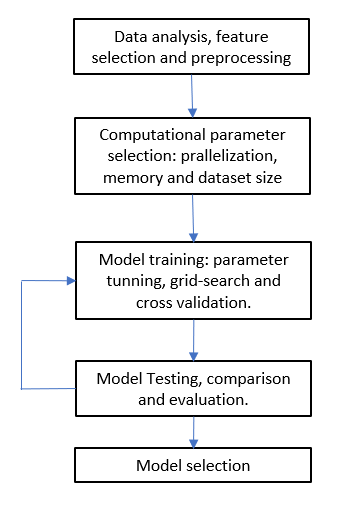
\includegraphics[width=0.5\linewidth]{TeX_files/Imagenes/general_met}
	\caption{General methodology for the project.}
	\label{fig:generalmet}
\end{figure}

1. Machine learning - training/testing 

\section{Data Overview}

The true redshift and the target redshif of BGS galaxies should in principle be equal, however, due to propagating error and missclasification in the data pipeline, the predicted redshift of the objects may have a deviation from its true value. Figure \ref{fig:bgs-z-truez} shows this relation, were a pattern between the two variables exist and is the reason to use machine learing. 
\begin{figure}[h!]
	\centering
	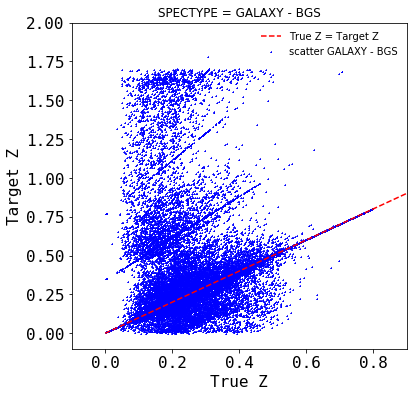
\includegraphics[width=0.7\linewidth]{TeX_files/Imagenes/BGS-z-truez}
	\caption{True and Target redsfhit relationship for BGS galaxies in the dataset. The red line indicates the line of calibration where the predicted redshift (target) is equal to the redshift of the galaxy (true) }
	\label{fig:bgs-z-truez}
\end{figure}

To explain the relation between the redshifts in Figure \ref{fig:bgs-z-truez}, we used the Flux G, R, Z, W1 and W2 as input variables from the dataset based on the effects of this variables on the variable $\alpha$ defined as
\begin{equation}
	\alpha = \frac{TRUEZ}{TARZ},
\end{equation}
as Figure \ref{fig:BGS-FLUX-ALPHA} shows. 
\begin{figure}[!htp]
	\centering
	\begin{subfigure}[t]{0.5\textwidth}
		\centering
		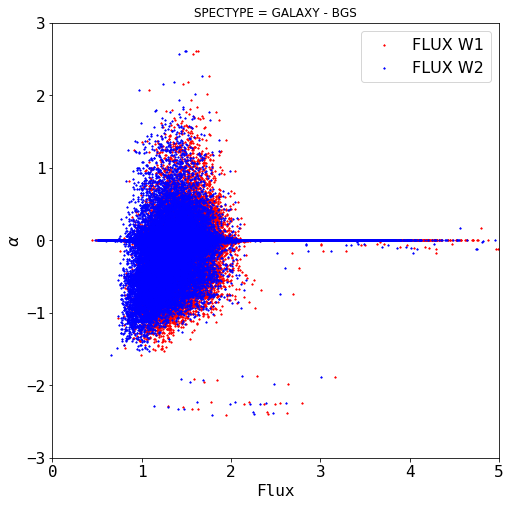
\includegraphics[height=3in]{TeX_files/Imagenes/BGS-FLUXW-ALPHA}
		\caption{}
	\end{subfigure}%
	\begin{subfigure}[t]{0.5\textwidth}
		\centering
		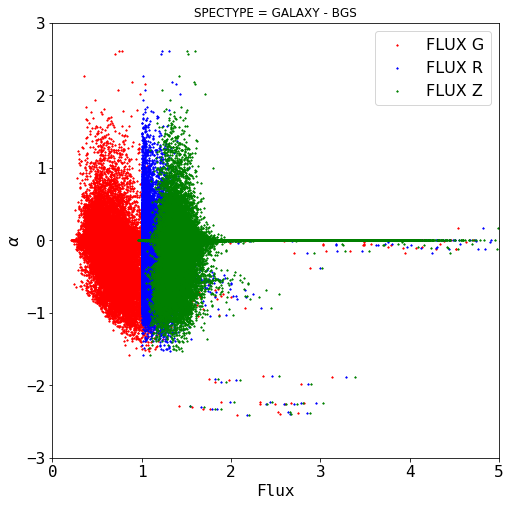
\includegraphics[height=3in]{TeX_files/Imagenes/BGS-FLUXRGZ-ALPHA}
		\caption{}
	\end{subfigure}
	\caption{Relation between fluxes, TRUEZ and TARZ. (a) $\alpha$ as a function of W1 and W2 fluxes. (b)$\alpha$ as a function of G, R and Z fluxes. $\log_{10}$ values presented.}
	\label{fig:BGS-FLUX-ALPHA}
\end{figure} 

Therefore, the selected variables for the machine learning model were: $\log_{10}(FLUX_G)$, $\log_{10}(FLUX_R),$ $\log_{10}(FLUX_Z),$  $\log_{10}(FLUX_{W1}),$  $\log_{10}(FLUX_{W2})$ and $TARZ$. For the predicted variable we chose $TRUEZ$, so our model takes in observational information \textit{and} DESI's predicted redshift to recover the true redshift of the object. 

\section{Results}
The dataset was split in a training set (75\%) and a test set (25\%). We trained three SVR and three KRR models on random subsets of the training set of size 100.000 each due to memory and training time problems, this subset was also subdivided in an 80-20 development - evaluation datasets for the application of grid search and cross-validation. The three KRR outperformed the three SVR models, then the KRR were ensemble together to produce a single oputput as Figure \ref{fig:ensemblemodel} shows.
  
\begin{figure}[h!]
	\centering
	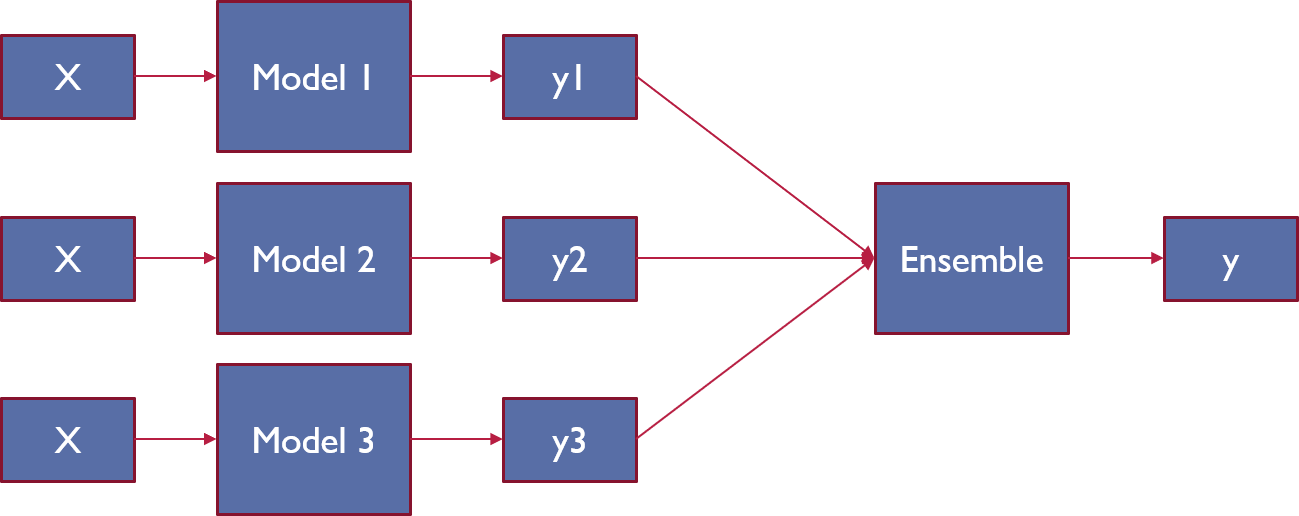
\includegraphics[width=1\linewidth]{TeX_files/Imagenes/ensemble_model}
	\caption{Graphic description of the ensemble model. It is formed based on the trained KRR models, each model previously trained on a random subset of size 100.000}
	\label{fig:ensemblemodel}
\end{figure}

Table \ref{table:test-result} shows the coefficient of determination, $r^2$ for each regression model on the testing(unseen) subset. 

\begin{table}[h!]
	\centering
	\begin{tabular}{|c|c|}
		\hline 
		Model & $r^2$ \\ 
		\hline 
		Model 1 & 0.958 \\ 
		\hline 
		Model 2 & 0.956 \\ 
		\hline 
		Model 3 & 0.962 \\ 
		\hline 
		Model avg & 0.962 \\ 
		\hline 
		Model max & 0.949 \\ 
		\hline 
		Model w & 0.983 \\ 
		\hline 
	\end{tabular} 
	\caption{Results on the \textbf{test} set for the three KRR model and the ensembles. Model w corresponds to training a linear model to find the best weight coefficients of each of the three models.}
	\label{table:test-result}
\end{table}

\section{Conclusions}

\end{document}
